\section{Finite approximation and one-objective exactness}
\label{sec:approximation}

The continuum in Theorem~\ref{thm:indispensable-rays} is necessary for
an exact strict description. For approximate descriptions of the closed
hull, a finite family suffices, and its required size can be quantified.
Throughout this section $r\geq2$, and $D_r$ and $\mathcal K_r$ retain
their meanings from Section~\ref{sec:infinite-aggregation}.
For a finite family $F\subset\mathcal K_r\setminus\{0\}$, put
\[
 P_F=\bigcap_{\lambda\in F}\{x\in\R^{2r}:f_\lambda(x)\leq0\},
 \qquad
 e_N=\inf_{|F|\leq N}d_H(D_r,P_F).
\]
Here $d_H$ is Euclidean Hausdorff distance, with value $+\infty$ for
unbounded $P_F$. Since $D_r\subseteq P_F$ and $D_r$ is compact,
$d_H(D_r,P_F)=\sup_{x\in P_F}\dist(x,D_r)$, also with this extended
value. Multipliers may be rescaled arbitrarily and may lie in the
interior of the good cone. The definition counts inequalities; it
does not assert that an optimal family attaining $e_N$ exists.

\begin{theorem}\label{thm:approximation-rate}
For every integer $N\geq2$ and every $r\geq2$,
\begin{equation}\label{eq:approximation-rate}
 \frac{\sqrt2}{2000N^2}
 \ \leq\ e_N\ \leq\
 \frac{5\sqrt2\,\pi^2}{16(N-1)^2}.
\end{equation}
Thus $e_N=\Theta(N^{-2})$, with constants independent of $r$.
Equivalently, as $\varepsilon\downarrow0$, a uniform Hausdorff
error at most $\varepsilon$ requires and suffices with
$\Theta(\varepsilon^{-1/2})$ good aggregations.
\end{theorem}

The rate concerns the good multipliers of this system: unlike
Theorem~\ref{thm:no-finite-quadratics}, the quantitative lower bound
does not cover arbitrary quadratic inequalities. The constants
in~\eqref{eq:approximation-rate} are convenient explicit bounds, not
claimed to be optimal.

More explicitly, put $c_0=\sqrt2/2000$ and
$B_0=5\sqrt2\pi^2/16$. Any family of at most $N\geq1$ cuts
whose error is at most $\varepsilon>0$ must have
$N\geq\sqrt{c_0/\varepsilon}$; the lower-bound proof below also
applies when $N=1$. Conversely, the equally spaced family with
$\lceil\sqrt{B_0/\varepsilon}\rceil+1$ cuts suffices, and its size
is less than $\sqrt{B_0/\varepsilon}+2$. This sufficiency uses an
explicit construction, not attainment of the infimum defining $e_N$.

\subsection{Angle sampling and a uniform radial correction}

For $x=(u,v)$ define
\[
 B(x)=\begin{pmatrix}
 1-\|u\|^2&u\transpose v-1/2\\
 u\transpose v-1/2&1-\|v\|^2
 \end{pmatrix},\quad
 q(\theta)=\begin{pmatrix}\cos\theta\\\sin\theta\end{pmatrix},\quad
 \lambda(\theta)=(\cos^2\theta,\sin^2\theta,2\sin\theta\cos\theta).
\]
The use of $\lambda(\theta)$ here is an angle parametrization of the
rays $\lambda(\tau)$ in Section~\ref{sec:infinite-aggregation}:
for $0<\theta<\pi/2$ the rays agree when $\tau=\cot\theta$.
The endpoints give the two coordinate rays. These rays generate
$\mathcal K_r$, so Theorem~\ref{thm:ball-hulls} gives
\begin{equation}\label{eq:angle-hull}
 x\in D_r\quad\Longleftrightarrow\quad
 h_x(\theta):=q(\theta)\transpose B(x)q(\theta)
 =-f_{\lambda(\theta)}(x)\geq0
 \quad(0\leq\theta\leq\pi/2).
\end{equation}
Only nonnegative directions $q(\theta)$ are tested: $B(x)$ need not
be positive semidefinite for $x\in D_r$.

\begin{lemma}\label{lem:angle-mesh}
Let $0=\theta_1<\cdots<\theta_N=\pi/2$, and let
$\Delta=\max_j(\theta_{j+1}-\theta_j)$. The relaxation $P_F$ using
$F=\{\lambda(\theta_j):1\leq j\leq N\}$ satisfies
\[
 d_H(D_r,P_F)\leq\frac{5\sqrt2}{4}\Delta^2.
\]
\end{lemma}
\begin{proof}
The endpoint cuts give $\|u\|,\|v\|\leq1$ on $P_F$.
On this product of balls, the diagonal entries of $B(x)$ lie in
$[0,1]$ and its off-diagonal entry lies in $[-3/2,1/2]$.
The maximum absolute row sum therefore gives
$\|B(x)\|_{\mathrm{op}}\leq5/2$. Since $q''=-q$,
\[
 h_x''(\theta)=2q'(\theta)\transpose B(x)q'(\theta)
                 -2q(\theta)\transpose B(x)q(\theta),
 \qquad |h_x''(\theta)|\leq10.
\]
If a minimizing angle is an endpoint, the minimum is nonnegative.
Otherwise its first derivative is zero, and a mesh point lies within
$\Delta/2$. Taylor's upper bound at that mesh point, whose value is
nonnegative, gives
\begin{equation}\label{eq:angle-defect}
 h_x(\theta)\geq-a\quad\hbox{for all }\theta,
 \qquad a=5\Delta^2/4.
\end{equation}
This estimate holds at every point of $P_F$.

Now $B(0)=\begin{pmatrix}1&-1/2\\-1/2&1\end{pmatrix}
\succeq I_2/2$ and
\[
 B(sx)=s^2B(x)+(1-s^2)B(0)\qquad(0\leq s\leq1).
\]
Choose $s=(1+2a)^{-1/2}$. Equations~\eqref{eq:angle-hull}
and~\eqref{eq:angle-defect} imply
$h_{sx}(\theta)\geq-s^2a+(1-s^2)/2=0$, so $sx\in D_r$.
Since $\|x\|\leq\sqrt2$,
\[
 \dist(x,D_r)\leq\|x-sx\|
 \leq\sqrt2\bigl(1-(1+2a)^{-1/2}\bigr)\leq\sqrt2 a.
\]
The last inequality follows from the tangent bound
$(1+2a)^{-1/2}\geq1-a$ for the convex function on $a\geq0$.
Taking the supremum proves the claim.
\end{proof}

Taking $N$ equally spaced angles gives
$\Delta=\pi/[2(N-1)]$ and proves the upper bound in
Theorem~\ref{thm:approximation-rate}, including $N=2$.
Exact rational coefficients give the same asymptotic rate.

\begin{corollary}\label{cor:rational-mesh}
For $N\geq3$ set $m=\lfloor(N-1)/2\rfloor$. The distinct multipliers
\begin{equation}\label{eq:rational-mesh}
 (m^2,j^2,2mj),\qquad(j^2,m^2,2mj),\qquad j=0,\ldots,m,
\end{equation}
define a relaxation using $2m+1\leq N$ cuts with
\[
 d_H(D_r,P_F)\leq\frac{5\sqrt2}{4m^2}.
\]
Every coefficient is an integer between $0$ and $2m^2$ and therefore
requires at most $2\lfloor\log_2 N\rfloor+3$ binary digits, hence
$O(\log N)$ bits.
\end{corollary}
\begin{proof}
The two lists share only the middle ray, and each multiplier satisfies
$\lambda_3^2=4\lambda_1\lambda_2$ exactly. Their angles are
$\arctan(j/m)$ and their reflections about $\pi/4$. They include
both endpoints and have gaps at most $1/m$, because $\arctan$ is
$1$-Lipschitz on $[0,1]$. Apply Lemma~\ref{lem:angle-mesh}.
For the digit count, $N<2^{\lfloor\log_2N\rfloor+1}$ gives
$2m^2\leq2N^2<2^{2\lfloor\log_2N\rfloor+3}$; the bound also
holds for the coefficient zero, encoded by one digit.
\end{proof}

The bit bound concerns the three multiplier coefficients, not the total
encoding of a quadratic in $2r$ variables or numerical solution error.
Preserving the rank-one identity in~\eqref{eq:rational-mesh} is useful:
independently rounding its three entries need not preserve goodness.

\begin{figure}[tbp]
 \centering
 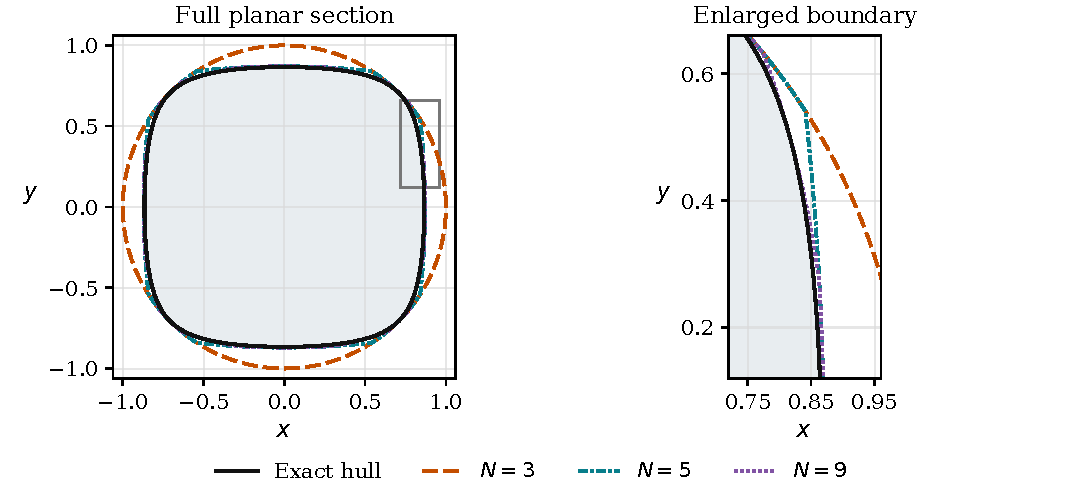
\includegraphics[width=\textwidth]{figures/finite-aggregation-slice.pdf}
 \caption{Sections by the plane $u=xe_1$, $v=ye_2$. The exact closed
 hull (black) is $(1-x^2)(1-y^2)\geq1/4$ inside $[-1,1]^2$.
 Colored curves bound the outer approximations from $N=3,5,9$ equally
 spaced angles in Lemma~\ref{lem:angle-mesh}; the right panel enlarges
 part of the first quadrant. The same planar sections occur for every
 $r\geq2$. The curves are computed from explicit radial formulas and
 illustrate the approximations; they are not estimates of their full
 Hausdorff errors.}
 \label{fig:finite-aggregation}
\end{figure}

\subsection{A lower bound allowing interior multipliers}

\begin{proof}[Proof of the lower bound in Theorem~\ref{thm:approximation-rate}]
Fix $F\subset\mathcal K_r\setminus\{0\}$ with $|F|\leq N$, and put
\[
 \eta=\frac1{400N^2},\qquad \epsilon=1/10.
\]
Use the $N+1$ parameters $\tau_j=1+j/N$, $j=0,\ldots,N$.
For each such $\tau$, choose $x_{\tau,\eta}=(u_{\tau,\eta},v_{\tau,\eta})$
with Gram matrix
\begin{equation}\label{eq:accuracy-gram}
 G_{\tau,\eta}=
 \begin{pmatrix}1-\epsilon/\tau&2/5-\eta\\
                 2/5-\eta&1-\epsilon\tau\end{pmatrix}.
\end{equation}
Here $0<\eta<1/10$, both diagonal entries are at least $4/5$,
and the off-diagonal entry has absolute value at most $2/5$.
Thus $\det G_{\tau,\eta}\geq12/25>0$. Such vectors exist in
$\R^2$ and embed in $\R^r$, with both norms at most one. They satisfy
\begin{equation}\label{eq:accuracy-values}
 f(x_{\tau,\eta})=(-\epsilon/\tau,-\epsilon\tau,\epsilon+\eta).
\end{equation}

Consider any $\lambda\in F$. If either $\lambda_1$ or $\lambda_2$
vanishes, goodness forces $\lambda_3=0$, and the nonzero cut is
strictly satisfied at every witness. Otherwise put
$t=\sqrt{\lambda_1/\lambda_2}>0$ and
$b=\sqrt{\lambda_1\lambda_2}$. If the cut excludes a witness,
then~\eqref{eq:accuracy-values} gives
\[
 \epsilon(\lambda_1/\tau+\lambda_2\tau-\lambda_3)
 <\eta\lambda_3.
\]
Using $\lambda_3\leq2b$ on both sides and dividing by
$\epsilon b$ yields $t/\tau+\tau/t<2a$, where $a=1+10\eta$.
If the same cut excludes a second parameter $\sigma$, adding the
two inequalities and applying the arithmetic--geometric mean
inequality gives
\[
 4a>(\tau+\sigma)\left(\frac{t}{\tau\sigma}+\frac1t\right)
 \geq\frac{2(\tau+\sigma)}{\sqrt{\tau\sigma}}.
\]
It follows that
\begin{equation}\label{eq:grid-exclusion}
 (\tau-\sigma)^2<4\tau\sigma(a^2-1)
 \leq16(a^2-1)
 =\frac4{5N^2}+\frac1{100N^4}<\frac1{N^2}.
\end{equation}
Distinct grid parameters differ by at least $1/N$. Thus one cut
excludes at most one of the $N+1$ witnesses. At most $N$ cuts
leave some $x_{\tau,\eta}$ in $P_F$. This finite pigeonhole
argument imposes no restriction on $t$ or extremality of $\lambda$.

For this witness the good multiplier
$\lambda_*=(\tau,1/\tau,2)$ has
$f_{\lambda_*}(x_{\tau,\eta})=2\eta>0$. Its leading matrix is
\[
 \begin{pmatrix}\tau&-1\\-1&1/\tau\end{pmatrix}\otimes I_r,
\]
which is positive semidefinite with operator norm
$\tau+1/\tau\leq5/2$. Hence
$\|\nabla f_{\lambda_*}(x)\|\leq5\sqrt2$ on the convex product
of the two unit balls. Both the witness and every $y\in D_r$
lie in that product, and $f_{\lambda_*}(y)\leq0$. The mean-value
inequality therefore gives
\[
 2\eta\leq f_{\lambda_*}(x_{\tau,\eta})-f_{\lambda_*}(y)
 \leq5\sqrt2\|x_{\tau,\eta}-y\|.
\]
Consequently
$d_H(D_r,P_F)\geq\sqrt2\eta/5$, proving the stated lower bound.
For an unbounded relaxation the bound holds with infinite left side.
\end{proof}

\subsection{Uniform objective gaps and an exact cut for one objective}

For a compact convex set $L$, write
$h_L(c)=\max_{x\in L}c\transpose x$. If $P_F$ is bounded, then
\begin{equation}\label{eq:hausdorff-support}
 d_H(D_r,P_F)=\sup_{\|c\|=1}\bigl(h_{P_F}(c)-h_{D_r}(c)\bigr).
\end{equation}
Indeed, choosing a closest point in $D_r$ bounds each support gap
above by the Hausdorff distance. Conversely, for $x\in P_F\setminus
D_r$ and its projection $y$ onto $D_r$, the unit vector
$c=(x-y)/\|x-y\|$ satisfies $h_{D_r}(c)=c\transpose y$ and
$h_{P_F}(c)\geq c\transpose x$. Taking the supremum gives the
reverse inequality; the case $P_F=D_r$ is immediate.

Thus Theorem~\ref{thm:approximation-rate} quantifies the worst gap
over unit linear objectives for one common bounded relaxation.
It applies to the final family even if the cuts were selected adaptively.
It does not give an iteration lower bound for solving one prescribed
objective. The next proposition makes that distinction explicit.

\begin{proposition}\label{prop:one-objective}
For every nonzero $c\in\R^{2r}$, there is a nonzero good multiplier
$\lambda\in\mathcal K_r$ such that
\begin{equation}\label{eq:one-objective}
 \min_{x\in D_r}c\transpose x
 =\min\{c\transpose x:f_\lambda(x)\leq0\}.
\end{equation}
Both minima are attained at a common point.
\end{proposition}
\begin{proof}
Let $F(x)=(f_1(x),f_2(x),f_3(x))$ and
$\mathcal K_r^*=\{z:\lambda\transpose z\geq0\text{ for all }
\lambda\in\mathcal K_r\}$. Convexity of every $f_\lambda$ for
$\lambda\in\mathcal K_r$ implies
\[
 \theta F(x)+(1-\theta)F(y)-F(\theta x+(1-\theta)y)
 \in\mathcal K_r^*\qquad(0\leq\theta\leq1).
\]
It follows directly that
\[
 E=\{(F(x)+z,c\transpose x+t):x\in\R^{2r},\
                            z\in\mathcal K_r^*,\ t\geq0\}
\]
is convex. It has nonempty interior because
$\mathcal K_r^*$ contains $\R^3_+$, and $t$ may increase freely.
The closed good-aggregation description of $D_r$ says that
$x\in D_r$ exactly when $-F(x)\in\mathcal K_r^*$.
Let $v=\min_{D_r}c\transpose x$ and choose a minimizer $x_*$,
which exists by compactness. Then $(0,v)\in E$, whereas
$(0,v-\delta)\notin E$ for every $\delta>0$.
Thus $(0,v)$ is a boundary point. A supporting hyperplane gives
a nonzero pair $(\lambda,\mu)$ satisfying
\[
 \lambda\transpose(F(x)+z)+\mu(c\transpose x+t)\geq\mu v
 \qquad(x\in\R^{2r},\ z\in\mathcal K_r^*,\ t\geq0).
\]
This supporting-hyperplane assertion does not require $E$ to be
closed: its nonempty interior has the same interior as its closure,
so one may support that closure at the included boundary point.
The recession directions $z,t$ and the bipolar theorem force
$\lambda\in\mathcal K_r$ and $\mu\geq0$.

For every nonzero $\lambda\in\mathcal K_r$,
\[
 f_\lambda(0)=-\lambda_1-\lambda_2+\lambda_3/2
 \leq-(\lambda_1+\lambda_2)/2<0.
\]
Evaluation at zero therefore rules out $\mu=0$. Normalize
$\mu=1$ to obtain
$f_\lambda(x)+c\transpose x\geq v$ for all $x$.
Evaluation at $x_*$, where $f_\lambda(x_*)\leq0$, gives
$f_\lambda(x_*)=0$. Also $\lambda\ne0$, since otherwise a
nonzero linear function would be bounded below on all of $\R^{2r}$.
For every $x$ satisfying $f_\lambda(x)\leq0$ we now have
$c\transpose x\geq v-f_\lambda(x)\geq v$, while $x_*$ attains
equality. Proposition~\ref{prop:ball-good-cone} ensures goodness.
\end{proof}

This is the usual strict-feasibility argument for conic convex duality,
specialized to the cone of convex aggregations; see
\citet[Section~5.9]{BoydVandenberghe2004}. The strict point is the
origin for the convex hull description, not for the original three
inequalities. Finding the objective-dependent multiplier can itself
require solving the original convex problem, and the proposition gives
no bound on that cost.

\subsection{Comparison with approximation theory}

The exponent two is familiar in convex approximation.
\citet{Rote1992} proves optimal $O(N^{-2})$ error bounds for
piecewise linear upper and lower approximations of univariate convex
functions on compact intervals with finite endpoint slopes, using
function values and supporting slopes, and treats
planar convex figures as well. This is particularly close context for
sampling a one-dimensional parameter family. His tangent-and-chord
approximations are different from the prescribed quadratic sublevel
sets considered here. The classical
polyhedral bounds of \citet{BronshteynIvanov1975}, and the modern
area-sensitive bounds and comparison in \citet[Section~1 and
Theorems~1--2]{AryaFonsecaMount2025}, concern approximation by vertices,
linear halfspaces, or piecewise affine functions. They provide the
appropriate context for quadratic local error from sampling a
one-dimensional family; they do not directly give
Theorem~\ref{thm:approximation-rate} for this prescribed cone of
quadratic cuts in $2r$ dimensions.

What is specific here is a two-sided bound for the HHC example, with a
lower bound against arbitrary interior good multipliers, constants
uniform in the replication dimension, and an exact rational
construction. It measures the size of a finite family of good
aggregations as an alternative to the exact finite SDP lift in
Theorem~\ref{thm:ball-hulls}. We assert no new general approximation
exponent, optimal constant, numerical conditioning guarantee, solver
improvement, or runtime lower bound.
